	\begin{Huge}
			Medizininformatik
		\end{Huge}
		\begin{exampleblock}{\textcolor{white}{Was ist der Studiengang?}}
			Die Schnittstelle zwischen Klinikum, Ärzten und Medizintechnikern. Klassische Anwendungsbereiche sind E-Health, Medizinische Datenverarbeitung sowie die (Mit-)Entwicklung von Medizingeräten. Es wird ein stärkerer Fokus auf Biologie, Physik und medizinische Inhalte gelegt. Ein Schwerpunktfach gibt es nicht. Danach kann das Studium mit einem Master \\ (4 Semester Regelstudienzeit) weitergeführt werden.
		\end{exampleblock}
	
	\begin{block}{Welcher Teil macht wie viel im Studium aus?}
		\begin{figure}[h!]
			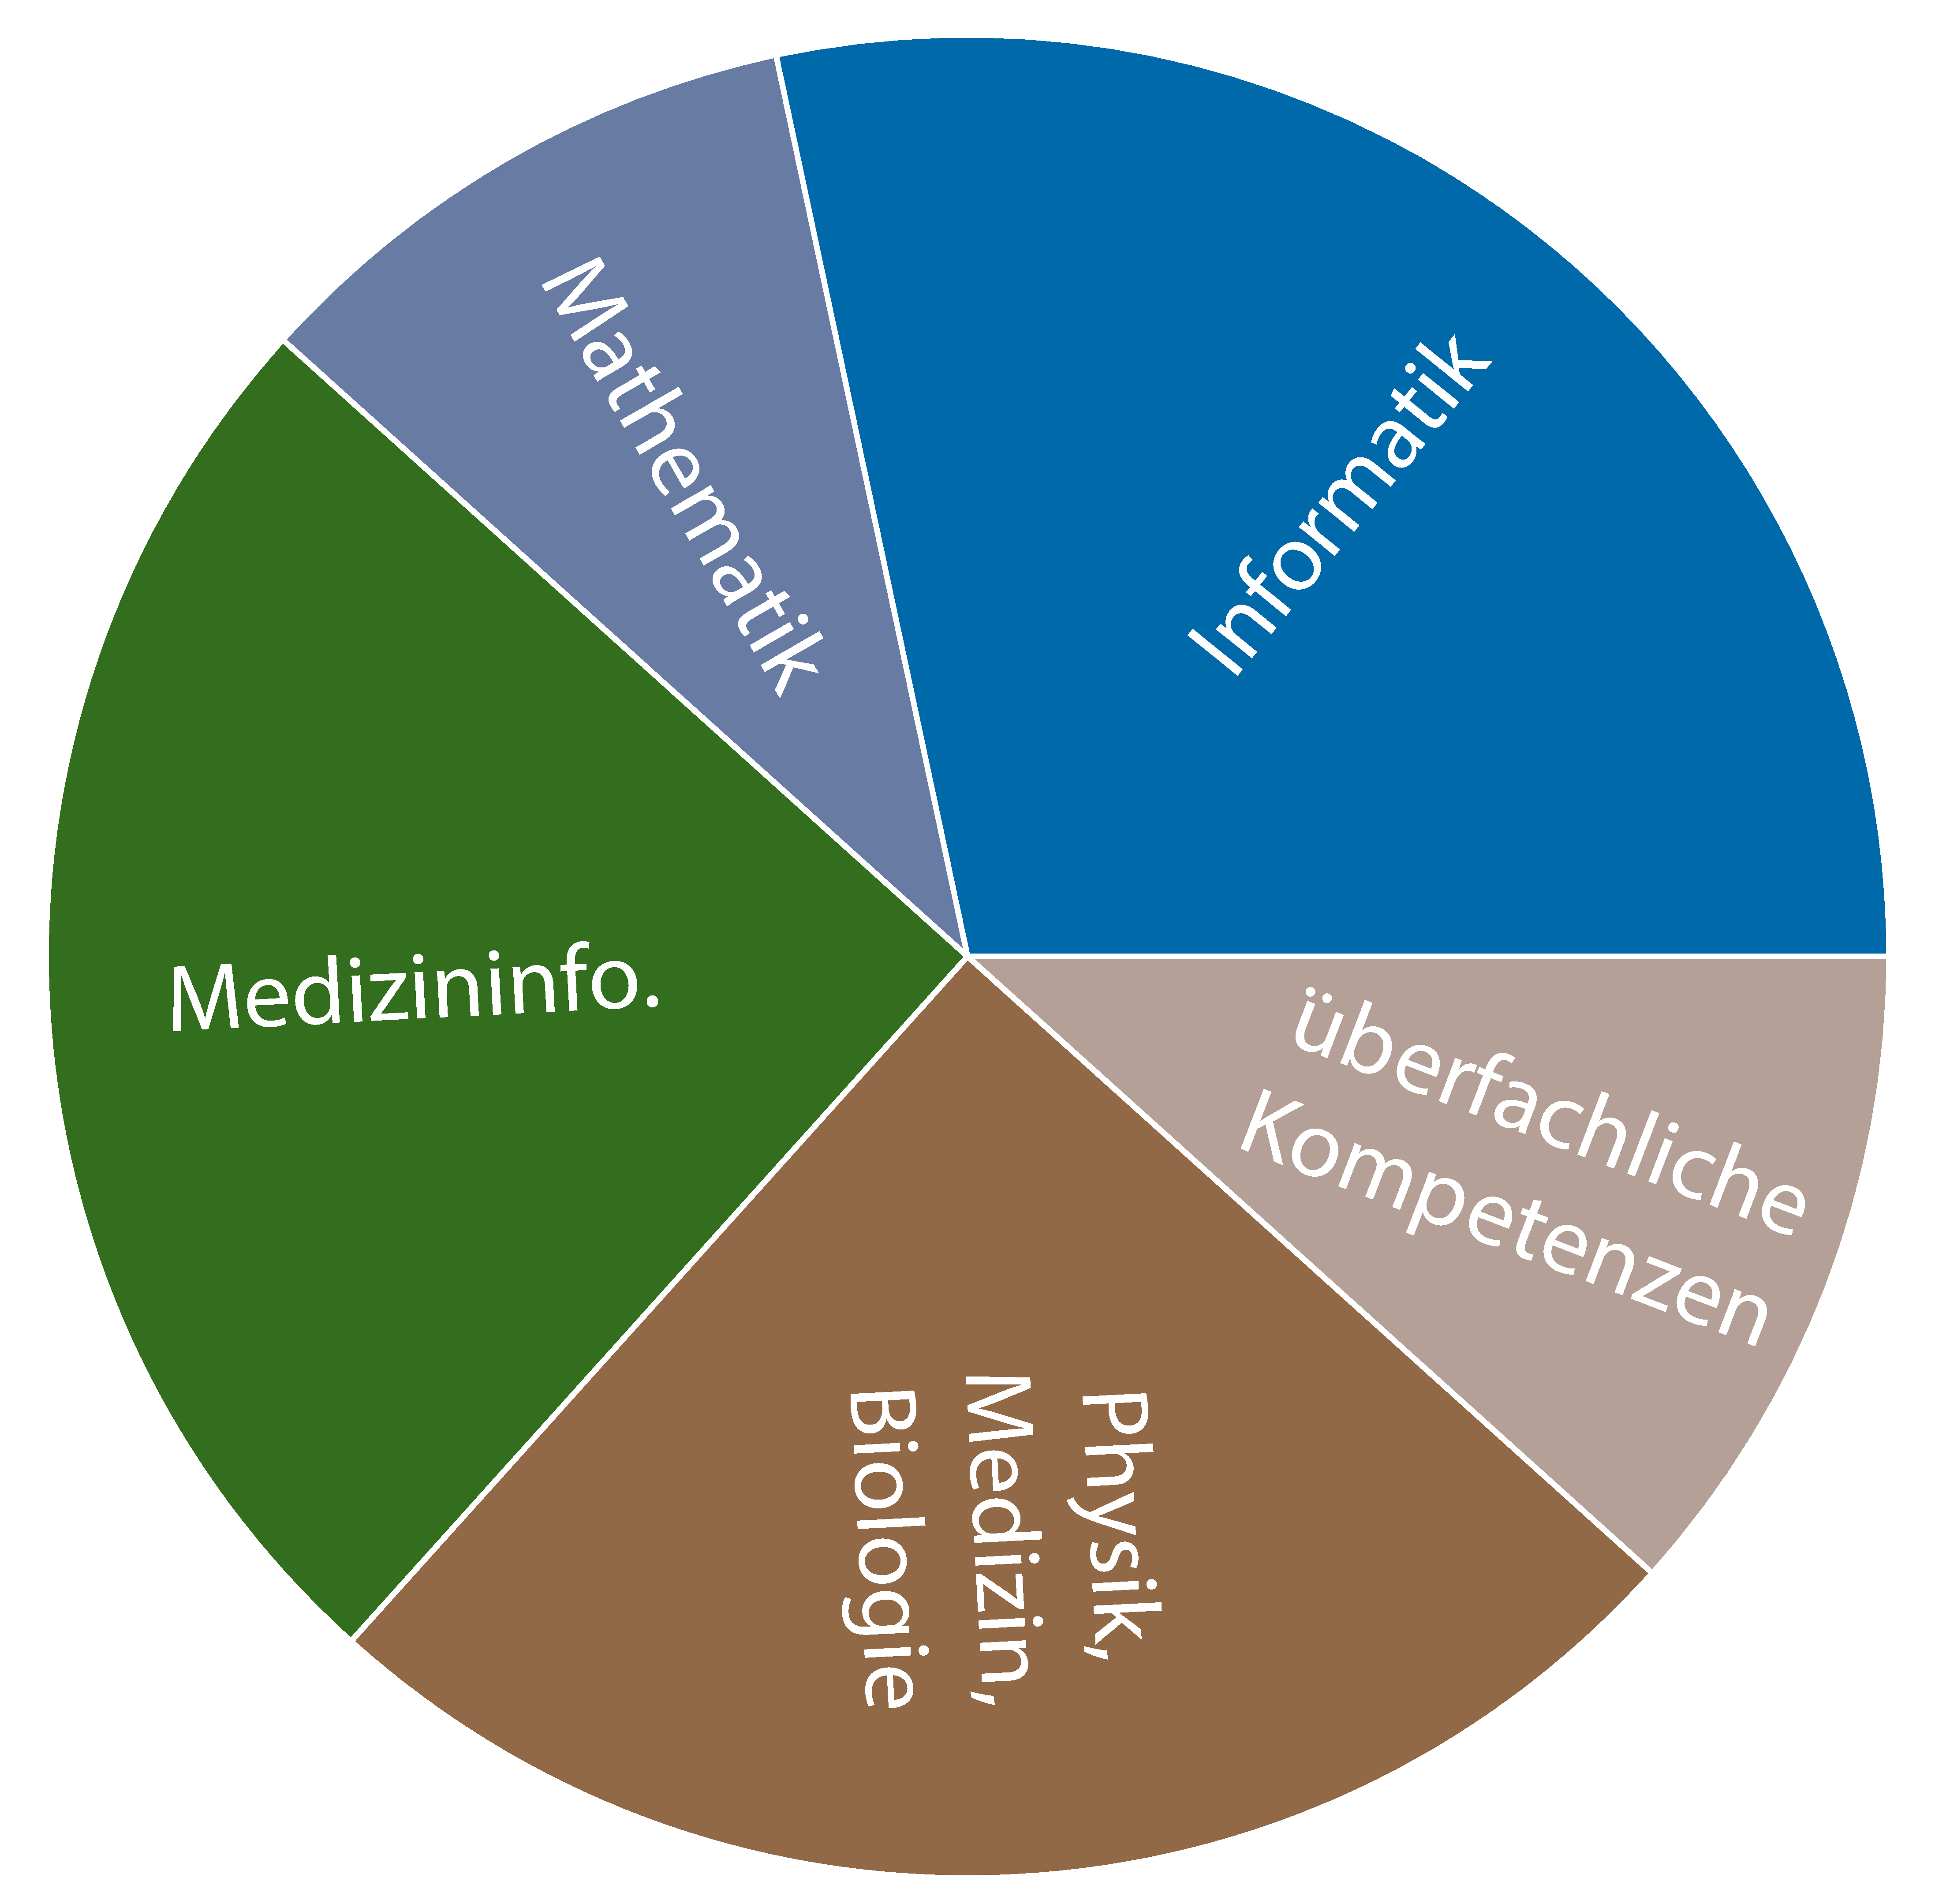
\includegraphics[width=0.4\textwidth]{charts/medizininformatik-Piechart.pdf}
			\caption{Verteilung der Themenbereiche über das komplette Studium}
		\end{figure}
	\end{block}
	
	\begin{block}{Was macht man in welchem Semester?}
		\begin{figure}[h!]
			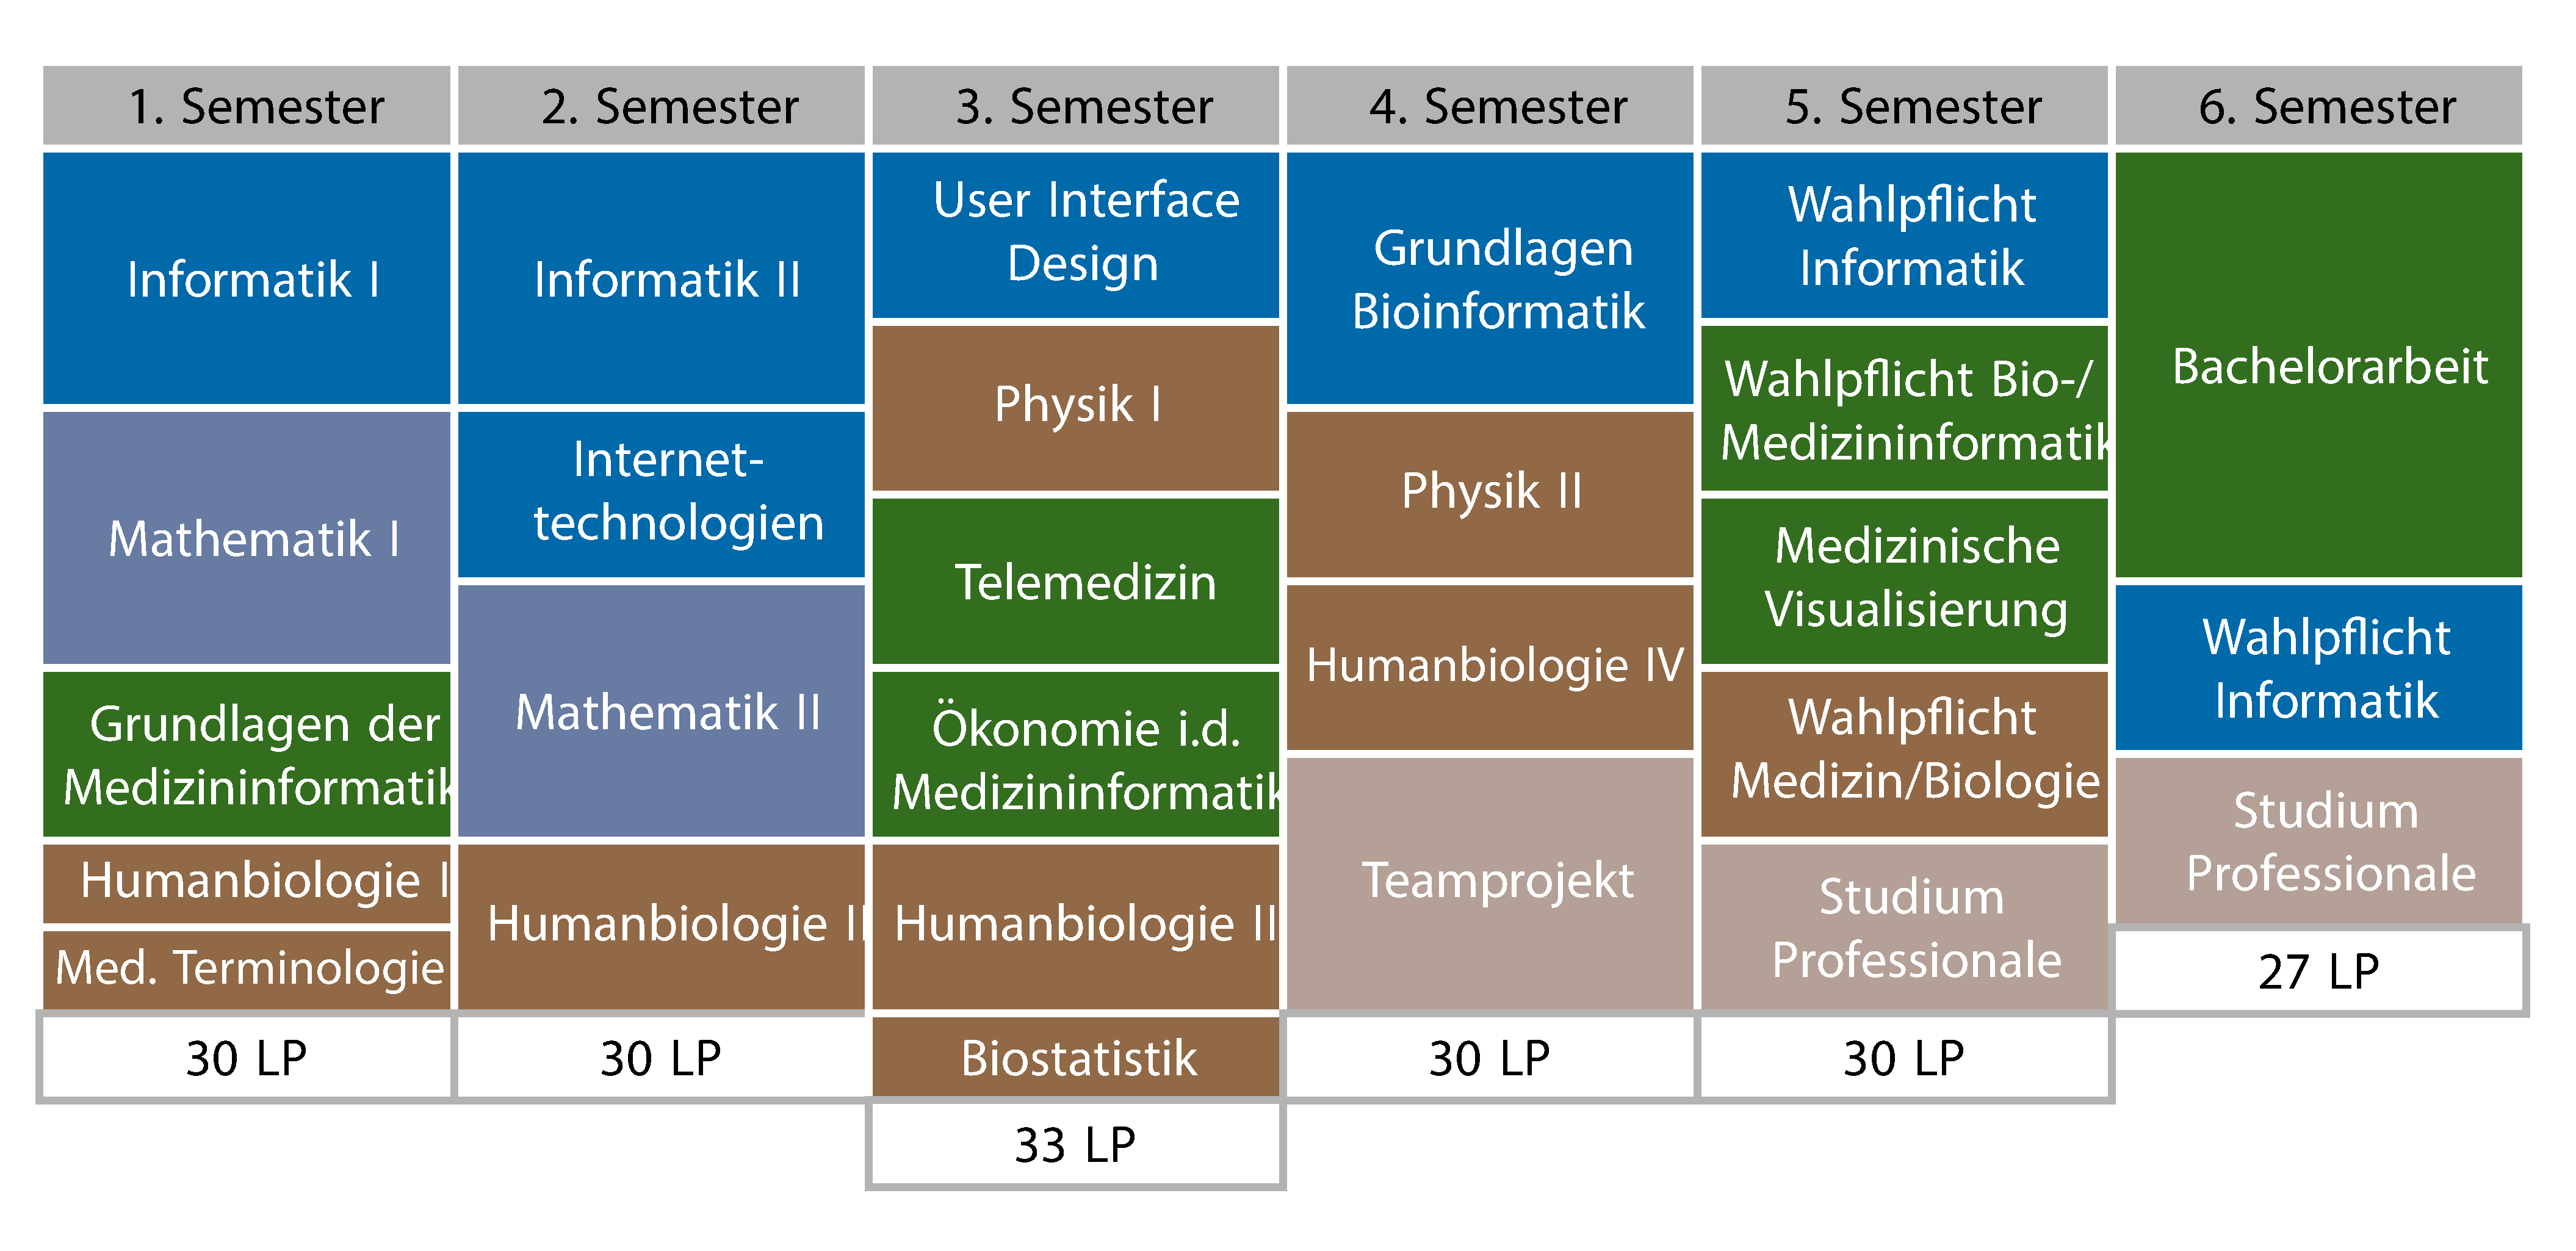
\includegraphics[width=\textwidth]{charts/medizininformatik_Studienplan_abWS18.pdf}
		\end{figure}
		Das 1. Semester ist nach Plan ein Wintersemester, der Studienbeginn ist hier auch nur zum Wintersemester möglich. 
		Dieser Verlauf ist lediglich ein Vorschlag und kein bindender Studienplan. Es empfiehlt sich jedoch, den Plan einzuhalten, wenn man in Regelstudienzeit studieren möchte.
	\end{block}
\vfill
\begin{flushright}
	
\includegraphics[width=0.4\textwidth]{fsilogo.pdf}
\end{flushright}